%% This is file `DEMO-TUDaSciPoster.tex' version 3.23 (2022/03/21),
%% it is part of
%% TUDa-CI -- Corporate Design for TU Darmstadt
%%
% !TeX program = lualatex
%%

\documentclass[
	accentcolor=3c,
%	boxstyle= boxed, % Boxen mit abgerundeten Ecken, farbigem Titelblock
	boxstyle=colored, % Boxen mit farbigen Titelblock, keine vertikalen Linien
%	boxstyle=default % Voreinstellung, ohne Farbe, ohne vertikale Linien
%	logofile=example-image, %Falls die Logo Dateien nicht vorliegen
	colorback=false,
	title=small
	]{tudasciposter}

%Sprache
\usepackage[ngerman,main=english]{babel}
\usepackage[autostyle]{csquotes}


\usepackage{multicol}
\usepackage{booktabs}
\usepackage{tabularx}
\usepackage[version=4,arrows=pgf-filled]{mhchem}
%\usepackage{mwe}
\usepackage{layouts}
\usepackage{vwcol}
\usepackage{paracol}

\def\app#1#2{%
	\mathrel{%
		\setbox0=\hbox{$#1\sim$}%
		\setbox2=\hbox{%
			\rlap{\hbox{$#1\propto$}}%
			\lower1.1\ht0\box0%
		}%
		\raise0.25\ht2\box2%
	}%
}
\def\approxprop{\mathpalette\app\relax}

\definecolor{tublau}{HTML}{005AA9}
\definecolor{tuorange}{HTML}{F5A300}
\definecolor{tu8b}{HTML}{EC6500}
\definecolor{turot}{HTML}{E6001A}
\definecolor{tulila}{HTML}{721085}
\definecolor{tutürkis}{HTML}{009D81}
\definecolor{tugrün}{HTML}{C9D400}
\definecolor{tu4b}{HTML}{99C000}
\definecolor{tudunkeltürkis}{HTML}{008877}

\makeatletter
\newcommand\thefontsize{The current font size is: \f@size pt}
\makeatother

\begin{document}
	\title{Two-layered Vectorial Kernel Models \\ for Detailed Surface Kinetics using a Goal-Oriented Approach}
	\author{\underline{Felix Döppel}\inst{1,*} Tizian Wenzel\inst{2} \and Robin Herkert\inst{2} \and Bernard Haasdonk\inst{2} \and Martin Votsmeier\inst{1,3}}
	\institute{\inst{1}Technische Universität Darmstadt, Darmstadt, Germany, \hfill \inst{*}Contact: felix.doeppel@tu-darmstadt.de \\
	\inst{2}Universität Stuttgart, Stuttgart, Germany, \\
	\inst{3}Umicore AG \& Co. KG, Hanau, Germany
	}
	%\inst kann in den Autor und Institutsfeldern genutzt werden um eine Zuordnung zu ermöglichen. Bei Nummerierung ist der Nutzer dafür verantwortlich Konflikte mit \thanks zu vermeiden.
	%\titlegraphic{\includegraphics[width=.5\linewidth]{example-image}}
%	\footerqrcode{https://www.chemie.tu-darmstadt.de/votsmeier/ak_votsmeier/index.en.jsp}
%	\footerqrcode{https://orcid.org/0000-0003-4733-9872}
	\footerqrcode{https://github.com/felix-doeppel/REACT_2023_Poster_VKOGA}
	\footer{
		[1] D. Micale, et al., \textit{Chemie-Ingenieur-Technik} \textbf{2022}, 1–19. \newline
		[2] G. Santin, and B. Haasdonk, in \textit{Model Order Reduction}, Vol. 1, De Gruyter \textbf{2019}\newline
		[3] T. Wenzel, F. Marchetti, and E. Perracchione, \textit{arXiv Preprint} \textbf{2023}. \newline
		[4] F. Döppel, and M. Votsmeier, \textit{Chemical Engineering Science}, \textbf{2022}, 262, 117964.
	}

%Instituts/Sponsorenlogos von links nach rechts
\footergraphics{
	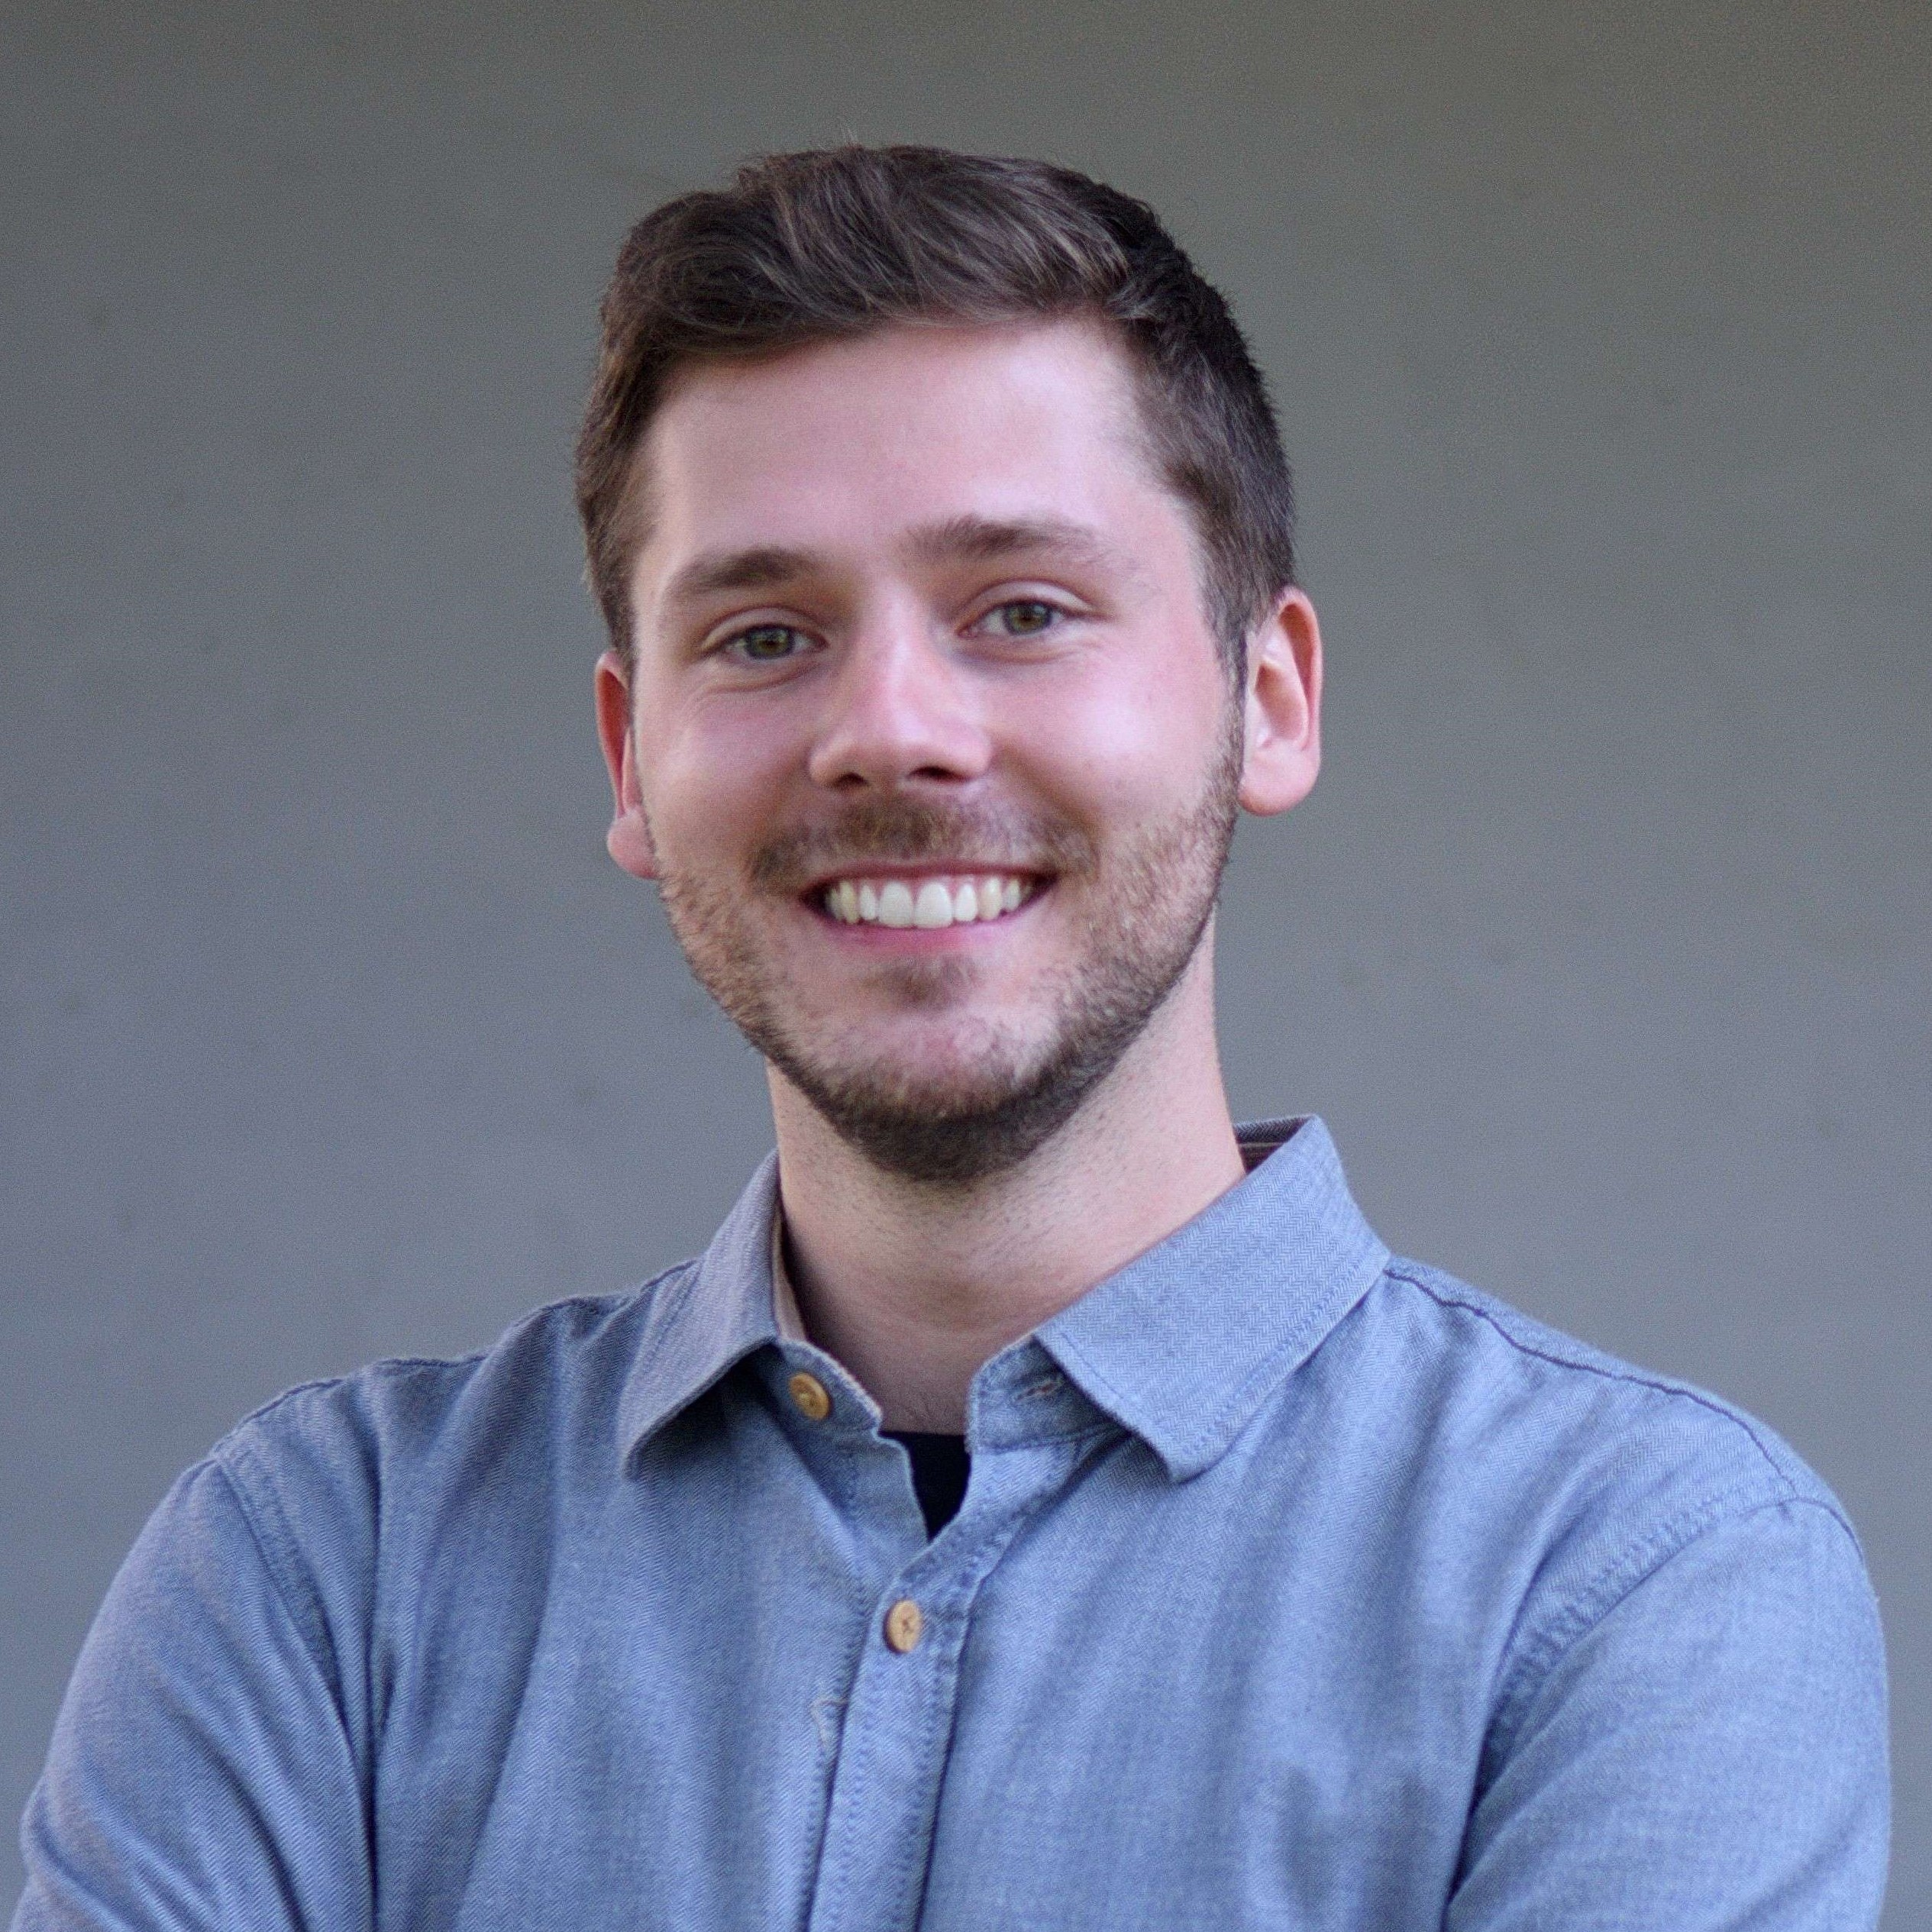
\includegraphics[height=\height]{abb/Profile_Pic_FD}
}

\begin{tcbposter}[
	poster={
		columns=8,
		rows=12,
		spacing=1cm,
%		showframe, %Gitter einblenden. Für Platzierung häufig hilfreich
	},]

\begin{posterboxenv}{name=GraphicalAbstract,column=1,row=1,span=8,rowspan=4}
%	textwidth in cm: \printinunitsof{cm}\prntlen{\textwidth}
	\centering
	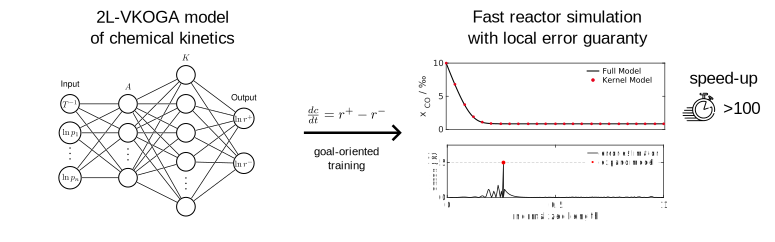
\includegraphics[width=\textwidth]{abb/GA_draft}
\end{posterboxenv}

\begin{posterboxenv}[title=1. Introduction]{name=intro,column=1,row=5,span=4,rowspan=2}
	\begin{itemize}
		\item \textbf{Detailed multi-scale modeling} provides valuable insights
		\item Kinetics are \textbf{computational bottleneck}\textsuperscript{[1]}
		\item Machine Learning surrogates speed up simulations
		\item Kernel models are deterministic and fast to train\textsuperscript{[2]}
	\end{itemize}
\end{posterboxenv}

\begin{posterboxenv}[title=2. Methods]{name=Methods,column=5,row=5,span=4,rowspan=2}
%	\begin{minipage}{0.675\textwidth}
	\begin{itemize}
		\item Extend novel, two-layered Kernel Models\textsuperscript{[3]} with a goal-oriented approach
		\item Embed chemical knowledge\textsuperscript{[4]} into the model structure %:\\Model $\ln r$ as $f(T^{-1}, \ln p_i)$
%		\item Select training data based on error in $\dot{s}$
%		\item Validate in plug-flow reactor simulations
		\item Model steady state solution of microkinetic model\textbf{}
		\item \textbf{Expand the model on-the-fly} if the error gets too high
	\end{itemize}
%	\end{minipage}
%	\begin{minipage}{0.3\textwidth}
%%		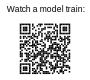
\includegraphics[width=.9\textwidth]{abb/QR_reference}
%	\end{minipage}
\end{posterboxenv}

\begin{posterboxenv}{name=Further Information,row=7,rowspan=4,column=5,span=4}
	\vspace{.5cm}
	\begin{multicols}{2}
%		\vspace{2cm}
		{\Large \centering Intelligent data sampling\\}
		\vspace{2cm}
		\includegraphics[width=.48\textwidth]{abb/VKOGA_hist}
		\captionof{figure}{
			The goal-oriented model automatically requests training data where the kinetics are harder\textsuperscript{[2]} to model (PEI~=~0.5).}
		\columnbreak
%		\vspace{2cm}
		{\Large \centering Increased accuracy\\}
		\vspace{2cm}
		\includegraphics[width=.48\textwidth]{abb/VKOGA_error} %{example-image-a}
		\captionof{figure}{The new model type is more accurate and needs fewer data.}
	\end{multicols}	
\end{posterboxenv}

\begin{posterboxenv}[title=3. Results]{name=Results,column=1,row=7,span=4,rowspan=4}
	\begin{itemize}
		\item Goal-oriented models \textbf{sample data where it's needed}
		\item Data utilization can be chemically understood
		\item Internal error estimator indicates accuracy during prediction
		\item Fast reactor simulations with a \textbf{local error guaranty}
	\end{itemize}
	\vspace{3cm}
%	\captionof{table}{Pro and contra of using Kernel Models instead of Neural Networks.}
	
	\begin{multicols}{2}
		VKOGA advantages
		\begin{itemize}
			\item[\textcolor{tudunkeltürkis}{\bullet}] Fast training
			\item[\textcolor{tudunkeltürkis}{\bullet}] Very data efficient
			\item[\textcolor{tudunkeltürkis}{\bullet}] Internal error estimator
		\end{itemize}
		\columnbreak
		Neural Network advantages
		\begin{itemize}
			\item[\textcolor{turot}{\bullet}] More literature available
			\item[\textcolor{turot}{\bullet}] Lots of implementations
			\item[\textcolor{turot}{\bullet}] GPU acceleration
		\end{itemize}
	\end{multicols}
	
%	\begin{tabularx}{\textwidth}{XX}
%%		\toprule
%		VKOGA advantages & Neural Network advantages \\ 
%		&\\
%		fast training & less accurate \\ 
%		very data efficient & fewer libraries/literature available\\
%		internal error estimator & no GPU implementation\\		
%%		\bottomrule
%	\end{tabularx}%
	


\end{posterboxenv}

\begin{posterboxenv}[title=4. Conclusion]{name=Conclusion,column=1,row=11,span=8,rowspan=2}
\begin{multicols}{2}		
	\begin{itemize}
		\item Goal-oriented approach leads to intelligent data sampling
		\item Two-layered models are more accurate and require less data
		\item Model training is very fast
		\item Reactor simulations are accelerated significantly
		\item Precision guaranty due to internal error estimator
	\end{itemize}
\end{multicols}

\end{posterboxenv}

\end{tcbposter}

\end{document}


